\section{(4pts)}
Plot the vertical acceleration versus time. Using your plot:
Calculate the damping ratio using the logarithmic decrement. Use a set of peaks 
away from the beginning of the measured response due to the initial lateral motion of the 
platform when it is released.

\begin{figure}[h]
    \centering
    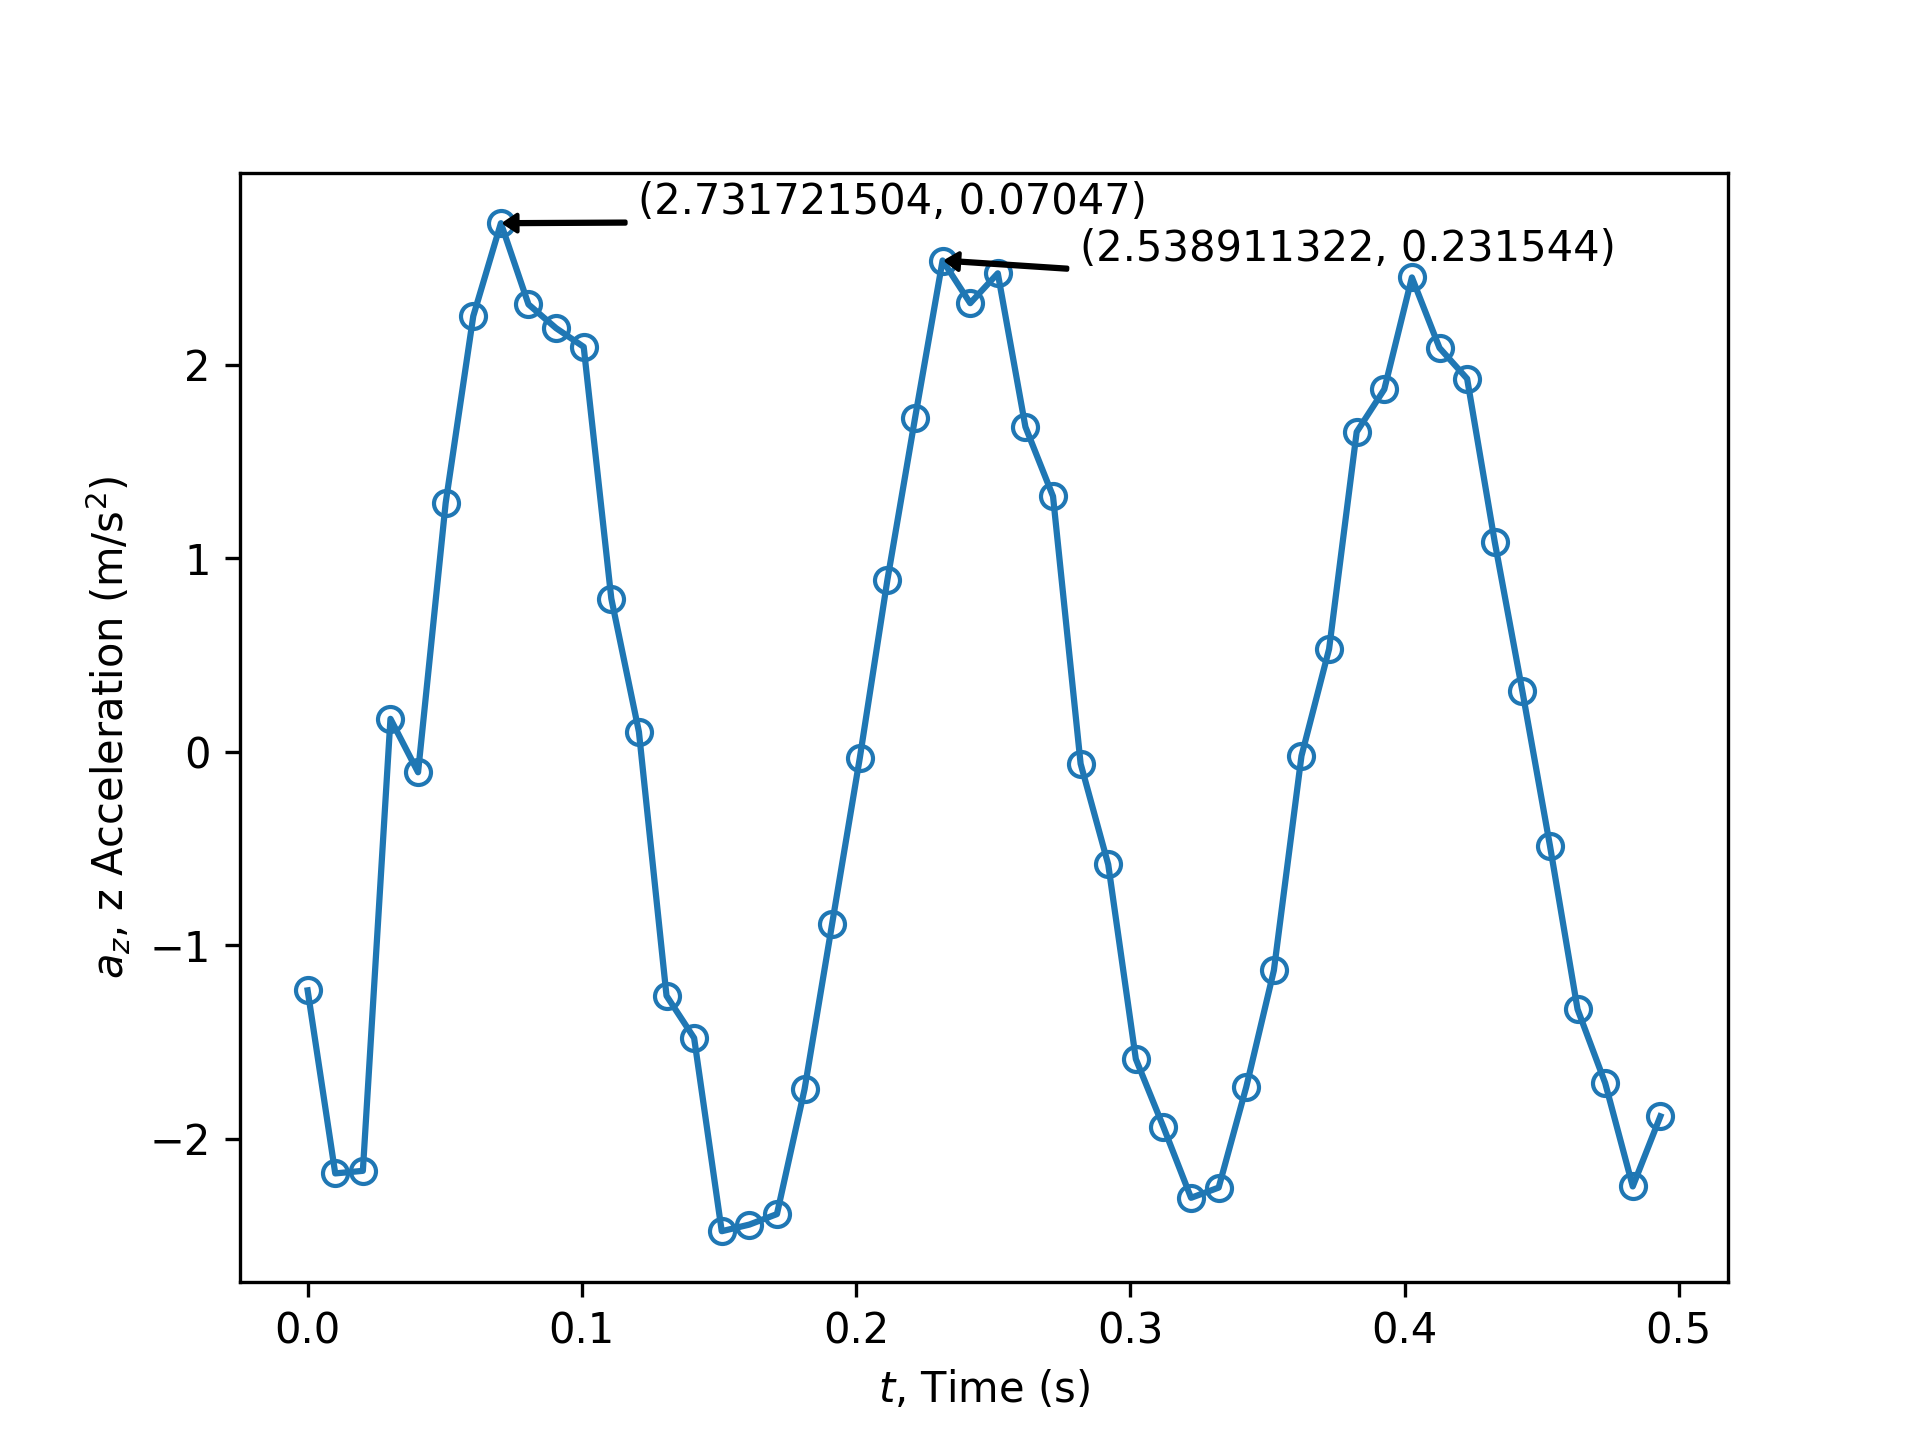
\includegraphics[width=0.5\textwidth]{Questions/Plots/z_acceleration.png}
    \caption{Vertical (z) acceleration of the platform after initial excitation.}
    \label{fig:z_acceleration}
\end{figure}    

Using the logarithmic decrement method,
\begin{align*}
    \delta &= \frac{1}{n} \ln\left(\frac{z_0}{z_n}\right) \\
    &= \frac{1}{1} \ln\left(\frac{2.731721504}{2.538911322}\right) \\
    &= 0.07320
\end{align*}
then,
\begin{align*}
    \zeta &= \frac{\delta}{\sqrt{4\pi^2 + \delta^2}} \\
    &= \frac{0.07320}{\sqrt{4\pi^2 + 0.07320^2}} \\
    &= 0.01165
\end{align*}




